\chapter{Transition Metal Systems Benchmark}
\label{ch:benchmark}
\section{Introduction}
I participated in a large multi-institutional collaboration that used 21 different electronic structure methods
on 21 transition metal atoms, ions and oxides, each of them for basis sets ranging from $d\zeta$ to $5\zeta$.
The goal of the project was to have 3 methods that provide essentially exact energies for these systems
(within the chosen basis sets) but at a cost that scales exponentially with system size, and use these
energies to assess the accuracy of 18 other methods that are approximate but exhibit better scaling.
My role in the project was to provide the SHCI energies (one of the 3 methods capable of providing the
exact energies, and in fact the only method that was able to compute all the systems for all the basis sets).

%There are many, not always mutually exclusive, approaches to dealing with the dimensionality: truncation of the wave function space through variational \textit{ansatz}, one-particle Green function approaches, density functional theory, Monte Carlo sampling, and embedding techniques. 
%The techniques vary dramatically in their computational cost and accuracy, and the degree to which they approximate the exact electronic structure solution.
%However, most studies\cite{bauschlicher_theoretical_1995,furche_performance_2006,doblhoff-dier_diffusion_2016,verma_assessment_2017,xu_practical_2015,minenkov_troubles_2016,thomas_accurate_2015} compare to experimental values,\cite{page_completing_1990} which can be subject to fortunate cancellation of error since all experimental results are differences in energies.
%
%In this manuscript, we apply a diverse array of 21 established and emerging approaches to a test set of small, realistic transition metal systems. 
%Each technique was implemented by an expert, and the Hamiltonian was carefully controlled to ensure that all calculations were performed on precisely the same system.  
%This approach allows us to directly assess methodological differences without confounders such as different Hamiltonians or other system-level approximations, and has proven highly relevant for previous benchmarks such as the hydrogen chain.\cite{Motta17} 
%For these systems, we achieve convergence of exponentially scaling but systematically convergeable methods at the order of 1 mHartree, or about 300 K, establishing a reliable reference on realistic Hamiltonians with complex atoms.
%We then assess the accuracy of more approximate approaches for computing the total energy of atoms and molecules, which allows some assessment of transferability of performance. 
%Finally, we study how errors in the solution of individual quantum systems translate into physical observables based on differences, and compare the high accuracy results to experiment. 


\section{Methods} 

\begin{table}
\caption{A list of abbreviations used in this benchmark.
Details are available in the Supplementary Information.
In Column A, the maximum basis set performed by that method for the transition metal atoms is listed, and in Column B the same for the monoxide 
molecules. }\label{table:abbreviations}
\begin{tabular} {l|p{0.5\columnwidth}|c|c}
Abbreviation & Method & A & B \\
\hline
AFQMC(MD) & Auxilliary field quantum Monte Carlo\cite{ShiweiPhaseless,Mario-WIRES-2018} & 5 & 5\\
iFCIQMC & Full configuration interaction quantum Monte Carlo & q & d\\
DMRG & Density matrix renormalization group & t & d \\
SHCI & Semistochastic heatbath configuration interaction & 5 &5 \\
CCSD(T) & Coupled cluster with singles, doubles, and perturbative triples\cite{bartlett_coupled-cluster_2007} & 5 & 5 \\
SEET(FCI/GF2) & Self-energy embedding theory & q & q \\
CISD & Configuration interaction with singles and doubles & 5 & 5 \\
QSGW & quasiparticle self-consistent GW approximation & t & t \\
HF+RPA & Hartree-Fock random phase approximation &t & t \\
SC-GW & Self-consistent GW approximation & d & - \\
GF2 & Second order Green function & q & q \\
CCSD & Couple cluster with singles and doubles\cite{bartlett_coupled-cluster_2007} & 5 &5 \\
MRLCC & multireference localized coupled cluster &5 & 5\\ 
DMC(SD)& Fixed node diffusion Monte Carlo with a single determinant nodal surface\cite{foulkes_quantum_2001,wagner_qwalk:_2009} & c & c\\
LDA & DFT in the local density approximation & 5 & 5\\
PBE & DFT in the PBE approximation &5 & 5  \\
HSE06 & DFT with the HSE06 functional &t & t\\
B3LYP & DFT with the B3LYP functional &5 & 5\\
SCAN & DFT with SCAN functional & 5 & 5\\
HF & Hartree-Fock & 5 & 5\\
    \end{tabular}
\end{table}

We consider transition metal systems, with the core electrons removed using effective core potentials\cite{trail_pseudopotentials_2013,trail_correlated_2015}. 
These potentials are an accurate representation of the core\cite{bennett_new_2017} for many-body simulations and allow all the methods considered in this work to be directly comparable. 
These potentials are available for Sc, Ti, V, Cr, Mn, Fe, and Cu, which defines our test set. 
We consider these transition metal atoms, their ions, and their monoxide molecules.
To simplify the comparison, the molecules were computed at their equilibirium geometry with bond lengths in {\AA} as follows: 
ScO: 1.668, TiO: 1.623,VO: 1.591, CrO: 1.621, MnO: 1.648, FeO: 1.616, CuO: 1.725.


Almost every electronic structure method works in a finite basis. 
Here, we follow the chemistry convention of defining an ascending basis set denoted by the $\zeta$ value, ranging from 2 to 5; i.e., d$\zeta$, t$\zeta$, q$\zeta$, and 5$\zeta$. 
For each system, we consider the first principles Hamiltonian projected onto that basis. 
%See the Supplementary Material for more details on the precise basis sets used in this study.
While these results are only comparable to experiment in the complete basis set limit (cbs), for each basis set there corresponds a projected Hamiltonian, which also has an exact solution. 
We thus can compare methods \textit{within a basis} since the Hamiltonian is defined precisely. 

\begin{figure}
\begin{center}
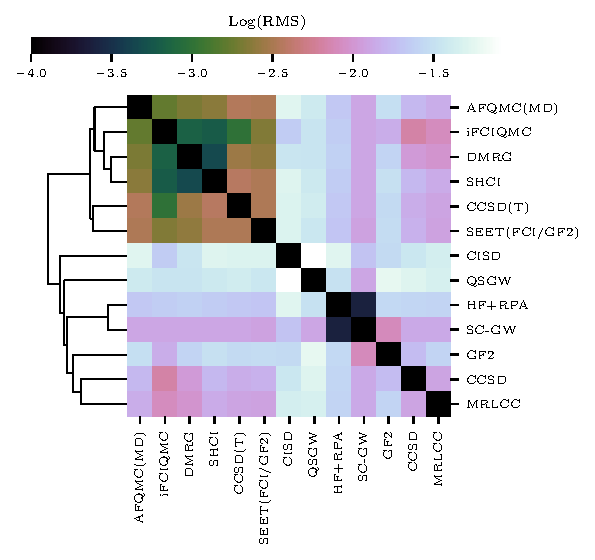
\includegraphics{figs/clustermap}
\caption{Cluster analysis of electronic structure methods in this work. 
The matrix values are the logarithm of the RMS deviation of the total energy in Hartrees (Eqn~\ref{eqn:rms}) between the two methods.}
    \label{fig:clustermap}
\end{center}
\end{figure}

The deviation in the total energy between two methods $m$ and $n$ is computed as
\begin{equation}
    \sigma(m,n) = \sqrt{\frac{\sum_{i \in \text{systems} } (E_i(n)-E_i(m))^2}{N}}.
    \label{eqn:rms}
\end{equation}
This is a measure of how well the output total energies between two methods agree; it is possible for two methods with large $\sigma$ to agree on energy \textit{differences}. 

To compare total energy between methods and systems in a consistent way, we use the concept of percent of correlation energy, commonly used in quantum chemistry:
\begin{equation}
    \text{\% correlation energy}(m) = 100 \times \frac{E_{HF} - E_{m}}{E_{HF}-E_{SHCI}},
    \label{eqn:correlation_energy}
\end{equation}
where $E_{HF}$ is the Hartree-Fock energy, $m$ stands for the method under consideration, and $E_{SHCI}$ is the total energy computed in the basis by the SHCI method.

Energy differences are assessed by considering the ionization potential of a transition metal $M$: $\text{IP}=E(M+) - E(M)$ and the dissociation energy of a metal oxide molecule $MO$: $\text{DE}=E(M)+E(O)-E(MO)$.
These quantities have been studied in detail for these systems in the past, for example Refs~\cite{bauschlicher_theoretical_1995,furche_performance_2006,doblhoff-dier_diffusion_2016,verma_assessment_2017,xu_practical_2015,bligaard_toward_2016,mardirossian_thirty_2017,minenkov_troubles_2016,thomas_accurate_2015,tew_explicitly_2016,johnson_communication:_2017}, among others. 
However, none of these previous studies have attained reference results as well-converged as the ones in this paper,
and none compare a large number of techniques on the same Hamiltonian.


\begin{figure*}
\begin{center}
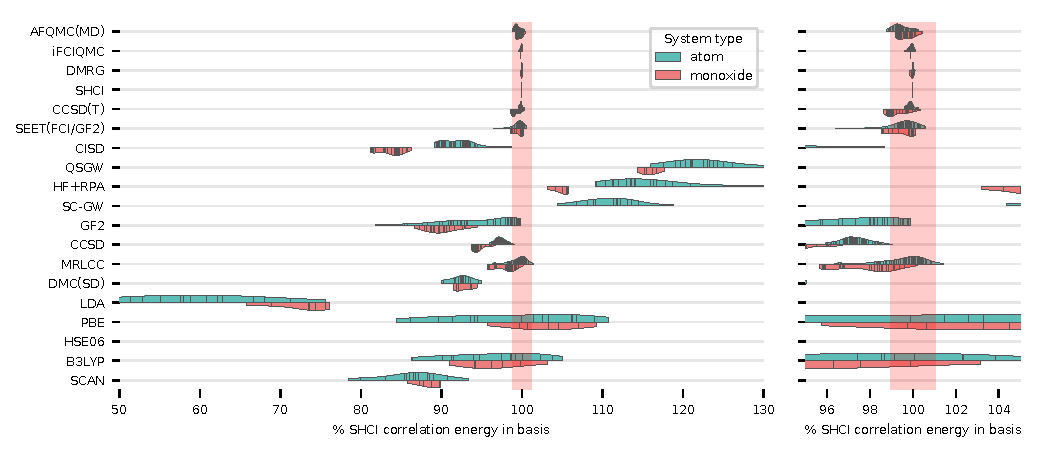
\includegraphics[width=\linewidth]{figs/correlation_energybar}
\caption{Kernel density estimation of the percent of the SHCI-computed correlation energy within each basis obtained by each of the methods in the benchmark set.
All basis sets available are plotted; individual data points are indicated by small lines.}\label{fig:correlation_energy}
\end{center}
\end{figure*}

In Table~\ref{table:abbreviations}, we classify the methods tested in this work. 
The ensemble of techniques includes many of the most common techniques to address the many-electron problem, as well as some emerging methods. 
We also include a few methods such as CISD which are no longer commonly used in calculations, but have historical relevance. 
The methods in this benchmark vary dramatically in their computational cost; the density functional theory methods required only a few minutes to complete the test set, while some of the more advanced techniques were not able to treat every basis for every system with the available amount of computer time.
The methods also scale very differently, ranging from $\mathcal{O}(N_e^3)$ to exponential in the number of electrons.



\section{Results} 

In Fig~\ref{fig:clustermap}, we show a cluster analysis of the total energy results using Eqn~\ref{eqn:rms} as the distance metric.
Three methods agree to better than 1 mHa on all attained basis sets and systems: DMRG, iFCIQMC, and SHCI\@. 
The iFCIQMC and DMRG techniques were not optimal for these systems, and so could only be completed to high accuracy for small basis sets.
These three methods each have single parameters that, when converged, theoretically should result in exact results. 
Because of this 3-fold agreement, we can take any of these results as the exact ground state energy in a given basis set to within about 1 mHa, which is approximately what is termed ``chemical accuracy.'' 
Among these three, only SHCI was performed for all basis sets and all systems and so we use that as the reference total energy.

\begin{figure*}
\begin{center}
    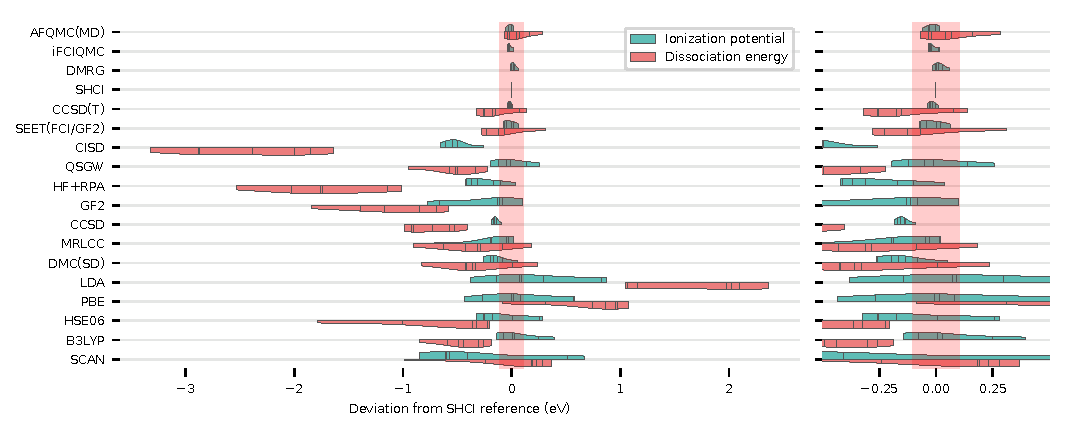
\includegraphics[width=\linewidth]{figs/BE_IP_SHCI}
    \caption{Kernel density estimation plot of binding energy and ionization potential of molecules and atoms to SHCI complete basis reference calculations. 
	Each technique is listed with the largest basis set available, so long as the basis set is triple-$\zeta$ or larger.
	Methods are ordered according to the clustering in Fig~\ref{fig:clustermap}.
 }\label{fig:be_ip}
\end{center}
\end{figure*}


Using this reference, one can compute the percent of correlation energy obtained by a given method, shown in Fig~\ref{fig:correlation_energy}. 
At 100\% of the correlation energy, the exact result is obtained. 
%This quantity is particularly useful since it is scale invariant and methods tend to cluster very well, with the exception of some of the density functionals. 
%We find that methods that work in a basis tend to obtain very similar percentages of the correlation energy across different basis sets.

%\begin{figure}
%\begin{center}
%    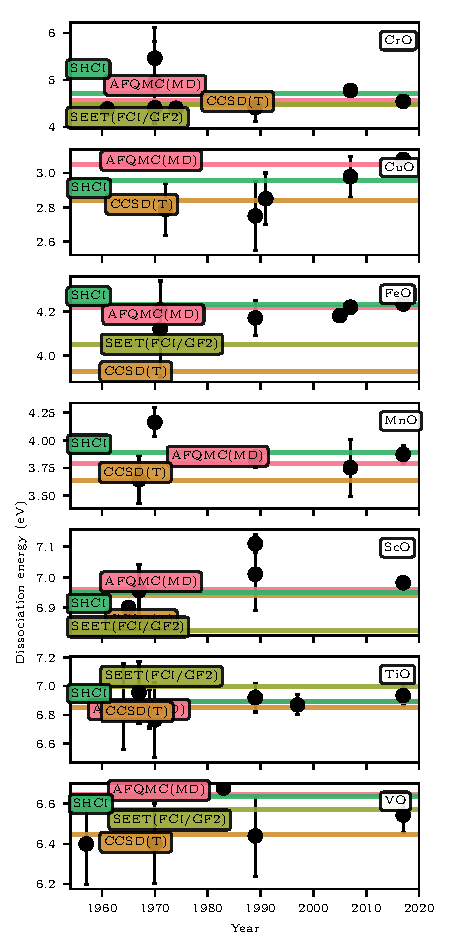
\includegraphics[width=0.5\linewidth]{figs/experimental_summary}
%    \caption{Comparison of highly accurate calculations in this work to experiment in the vqz basis. }
%    \label{fig:experiment}
%\begin{end}
%\end{figure}
%
%Comparing to experiment, the ionization potential of the large-basis SHCI results is in agreement with experiment with mean absolute deviation of 0.2 mHa, or 7 meV, so one could equivalently use experiment or the SHCI reference values. 
%The dissociation energy is more complex.
%In Fig~\ref{fig:experiment}, the high accuracy  estimates of the dissociation energy of the molecules is shown, compared to experimental values\cite{merer_spectroscopy_1989,carlson_electronic_1965,darwent_bond_1970,carlson_wavefunctions_1964,berkowitz_thermodynamics_1957,balducci_dissociation_1971,clemmer_reaction_1991}.
%For these systems, the experimental uncertainty of the dissociation energy is rather large compared to the agreement of the most accurate techniques in this benchmark.
%%We thus consider the deviation from the closest experimental value to a given method in Fig~\ref{fig:experiment}.
%We also should note that since we used effective core potentials to standardize the benchmark, there may be some small errors in comparing directly to experiment.
%However, we see no evidence that the potentials used are limiting the accuracy; the most accurate methods obtain results well within the experimental uncertainty.
%It is clear that all techniques depend on cancellation of errors; the uncertainty in basis set extrapolation of the total energy is $\sim$ 3 mHa $\simeq 0.1$ eV in the total energy, although these errors largely cancel in the ionization potential and the dissociation energy.
%
%
%\section{Conclusion} 
%
%We surveyed over 20 advanced many-electron techniques on precisely defined realistic Hamiltonians for transition metal systems. 
%For a given basis set, we achieved better than 1 mHa agreement on the total energy between high accuracy methods, which provides a \textit{total energy} benchmark for many-body methods. 
%To our knowledge, such an agreement on systems of this size is unprecedented for first principles calculations of transition metals.
%We were able to directly compare a method that works in the complete basis set, FN-DMC, to basis set methods, for transition metal systems, as well as provide a high quality reference for density functional theory calculations.
%The carefully defined Hamiltonian and reference total energy values enabled the comparison of approximate, but more computationally efficient, many-body techniques without the necessity of experimental references.
%This database is available to researchers, and we expect will be a signifant asset in the development of new more efficient and compact many-body computational frameworks. 
%Indeed several of the techniques tested are emerging, and benefited from the comparison.
%These systems are a useful test for future quantum computing algorithms for quantum simulation, since they are extremely well controlled. 
%To enable such comparisons, we include PySCF scripts that can execute the benchmark for any density functionals available in libxc\cite{marques_libxc:_2012}, and can export the many-body Hamiltonian for these systems.
%
%To avoid misinterpretation of the results, we make a comment here.
%In order to ensure the highest quality results and to converge the very high accuracy results, it was necessary to limit the number of systems on which this benchmark was performed. 
%The systems considered here are well-described using single reference techniques, and dynamic (short-ranged) correlation is extremely important to obtain accuracy.
%The performance profile will likely be different for other sets of chemical systems and so more benchmarking efforts of similar quality would be highly valuable.
%
%We have assessed the state of the art in achieving extremely high accuracy in realistic systems. 
%The benchmark set includes systems with large Hilbert spaces, around 10$^{44}$ dimensions.
%While these spaces are so large that a single vector cannot fit in any computer memory, they can be solved with small errors due to powerful compression of that space.
%However, the systematic techniques used in this work (DMRG, FCIQMC, and SHCI), while they were able to achieve excellent agreement, can only be applied to relatively small systems in the general case due to their computational cost.
%It is thus important to understand the errors in lower scaling techniques that can be applied to larger systems, and whether performance on small systems is also transferable to larger systems. 
%Our study takes an important step in that direction, since we were able to achieve converged results for both correlated atoms and molecules, and indeed we observed that some techniques perform differently on differently sized systems.

%\end{document}
%-----------------------------------
%\chapter{Transition Metal Systems Benchmark}
%I participated in a large multi-institutional collaboration that used 21 different electronic structure methods
%on 21 transition metal atoms, ions and oxides, each of them for basis sets ranging from $d\zeta$) to $5\zeta$).
%The goal of the project was to have 3 methods that provide essentially exact energies for these systems
%(within the chosen basis sets) but at a cost that scales exponentially with system size, and use these
%energies to assess the accuracy of 18 other methods that are approximate but exhibit better scaling.
%My role in the project was to provide the SHCI energies (one of the 3 methods capable of providing the
%exact energies, and in fact the only method that was able to compute all the systems for all the basis sets).
%\label{ch:benchmark}
%\section{Introduction}
%% \label{sec:benchmark:intro}
%Most electronic structure computation studies use experimental data for comparison and assessment.
%Since experimental observables are usually the differences between energies from theoretical models, many calculations could produce a good agreement to experiments by coincidence, or cancellations of errors, which are not well-examed.
%
%In this project~\cite{williams2019direct}, we apply a set of electronic structure methods to a set of small realistic transition metal systems.
%I perform the SHCI calculations and other calculations are performed by our collaborators, who are experts in the corresponding methods.
%For each system, the Hamiltonian is carefully controlled to ensure all the methods are calculating exactly the same system with the same system-level approximations.
%This approach allows us to access methodological differences directly without obfuscation from other errors.
%Table~\ref{table:abbreviations} presents the methods that we include in this project.
%
% \begin{table}
% \caption{A list of abbreviations used in this benchmark.
% In Column A, the largest basis set performed by that method for the transition metal atoms is listed, and in Column B the same for the monoxide
% molecules.~\cite{williams2019direct} }\label{table:abbreviations}
% \begin{tabular} {l|p{0.68\columnwidth}|c|c}
% Method & Full Name & A & B \\
% \hline
% AFQMC & Auxilliary field quantum Monte Carlo & 5 & 5\\
% iFCIQMC & Full configuration interaction quantum Monte Carlo & q & d\\
% DMRG & Density matrix renormalization group & t & d \\
% SHCI & Semistochastic heatbath configuration interaction & 5 &5 \\
% CCSD(T) & Coupled cluster with singles, doubles, and perturbative triples & 5 & 5 \\
% SEET & Self-energy embedding theory & q & q \\
% CISD & Configuration interaction with singles and doubles & 5 & 5 \\
% QSGW & quasiparticle self-consistent GW approximation & t & t \\
% HF+RPA & Hartree-Fock random phase approximation &t & t \\
% SC-GW & Self-consistent GW approximation & d & - \\
% GF2 & Second order Green function & q & q \\
% CCSD & Couple cluster with singles and doubles & 5 &5 \\
% MRLCC & multireference localized coupled cluster &5 & 5\\
% DMC & Diffusion Monte Carlo (single determinant) & c & c\\
% LDA & DFT in the local density approximation & 5 & 5\\
% PBE & DFT in the PBE approximation &5 & 5  \\
% HSE06 & DFT with the HSE06 functional &t & t\\
% B3LYP & DFT with the B3LYP functional &5 & 5\\
% SCAN & DFT with SCAN functional & 5 & 5\\
% HF & Hartree-Fock & 5 & 5\\
%     \end{tabular}
% \end{table}
%
%
%\section{Results}
%
%We use SHCI results as the reference values for these systems.
%The SHCI results are systematically converged to less than 1~mHa uncertainty.
%Fig.~\ref{fig:benchmark} and \ref{fig:benchmark_be} presents the results.
%
%\begin{figure}
%  \begin{center}
%  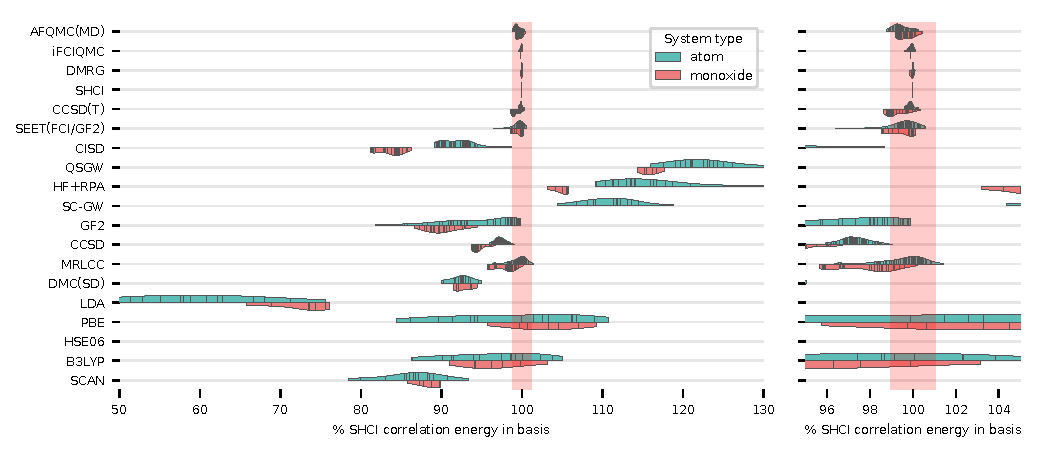
\includegraphics[width=\linewidth]{figs/correlation_energybar.pdf}
%  \caption{Percent of correlation energy recovered by approximate quantum chemsitry methods, using SHCI as a reference~\cite{williams2019direct}.
%}
%  \label{fig:benchmark}
%  \end{center}
%\end{figure}
%
%\begin{figure}
%  \begin{center}
%  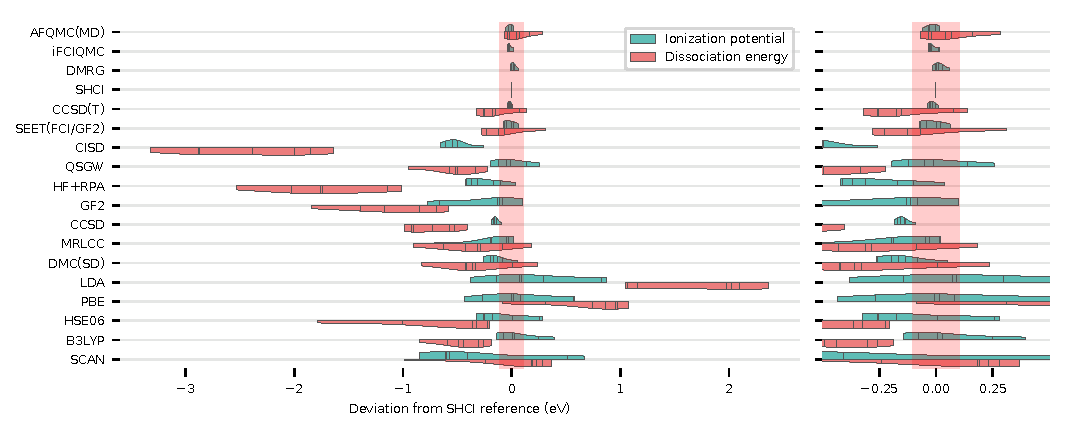
\includegraphics[width=\linewidth]{figs/BE_IP_SHCI.pdf}
%  \caption{Deviation of approximate quantum chemsitry methods from SHCI reference values~\cite{williams2019direct}.
%}
%  \label{fig:benchmark_be}
%  \end{center}
%\end{figure}

We can see that all the systematic methods, including FCIQMC, DMRG, and SHCI, agree exceptionally well with each other, for those basis sets where the FCIQMC and DMRG calculations were feasible.
This is as expected since they use the same Hamiltonian and all of these methods should give the full-CI energies without systematic errors.

However, systematic methods like these can only be applied to relatively small systems due to their high computational cost, so it is also important to study the errors in other more efficient methods.
These errors are often canceled out in previous studies when comparing to experimental data, and the results from our study make these errors directly accessible.

From these figures, we can see that both AFQMC and CCSD(T) give reasonably good agreement to the reference values and their computational costs increase much slower with the system size than the three essentially exact methods.
Other methods are much less accurate and thus may not produce reliable results for the energies.
%However, they may still provide reasonably accurate results for structural optimization.
However, they may still provide sufficient accuracy for some systems.
%reasonably accurate results for structural optimization.

In many cases, using less accurate methods can be the only option due to the high computational cost of more accurate methods.
In such cases, benchmark results from some sample systems of similar kind can provide useful information on which approximate method to choose.
